\chapter{A PERFORMANCE COMPARISON OF ADVANCED PLLs FOR GRID SYNCHRONIZATION} 
\label{3.Chap:PLL}
\section{INTRODUCTION} 
In Chapter \ref{2.Chap:DOCIntro}, a comprehensive discussion on the operating principle of the UPQC has been provided, specifically focusing on the implementation of both back-to-back and dual-output converters. Additionally, an extensive literature survey exploring various control strategies for generating reference quantities and control techniques has been included. The accurate estimation of the grid voltage phase angle is crucial for generating reference quantities, and the widely used method for this is the synchronous reference frame phase-locked loop (SRF-PLL). However, it is important to note that the dynamic performance of the SRF-PLL is optimal only when the grid voltages are balanced and free from distortion \cite{844502}. With the increasing integration of renewable energy sources (RESs) and the utilization of nonlinear loads in the distribution system, issues such as phase angle jumps, harmonics, and distortions in grid voltage can arise. Under such conditions, the dynamic performance of the SRF-PLL with high bandwidth deteriorates. To address this problem, one possible approach is to select a low bandwidth for improved performance, but this compromises the response speed, resulting in slower dynamic response. 

To accurately extract phase angle information from the distorted grid voltages, while maintaining zero steady-state error and achieving a fast response, it is necessary to pass the fundamental frequency positive sequence (FFPS) components through the SRF-PLL. In the literature, there are various methods available for extracting FFPS components, which can be broadly classified into two categories.

The first method is based on notch filters using the instantaneous symmetrical components theory (ISCT). By employing notch filters, the fundamental and quadrature components of the signals are extracted, and then the positive sequence components are derived using the ISCT. The second method utilizes delay operators, which inherently possess filtering capabilities. In this approach, quadrature signals can be generated by applying delay operators to each phase. However, it is worth noting that this method may result in increased execution time for digital simulators due to the higher demand for delay operators. Examples of the former method include enhanced PLL (EPLL) and second-order generalized integrator (SOGI). On the other hand, examples of the latter method include cascaded delayed signal cancellation (CDSC) and multiple delayed signal cancellation (MDSC) methods.

In \cite{1318659}, three EPLLs are employed, one for each phase, to extract the FFPS components. A fourth EPLL is employed to extract the phase angle of the grid voltage. The EPLL's performance remains robust in the face of frequency variations due to its frequency adaptive notch filter characteristics. To reduce the number of EPLLs employed, a dual EPLL (DEPLL) is proposed in the $\alpha \beta$  reference frame \cite{4153695}. This proposal assumes that the $\alpha \beta$  components of grid voltages are quadrature to each other. However, this assumption is no longer valid in unbalanced grid systems. To overcome this limitation, the second-order generalized integrator (SOGI) is suggested as a quadrature signal generator (QSG) \cite{1711988}. In recent years, PLLs based on SOGI, CDSC, and MDSC have gained popularity due to their individual advantages. However, each PLL approach has its own drawbacks. This chapter provides a concise review of these PLLs, explaining their basic principles, concepts and performance comparison. 
\vspace*{-.5cm}
\section{REVIEW ON ADVANCED PLLs}
This section presents a brief overview of SOGI, CDSC and MDSC based PLLs.
\vspace*{-1.5cm}
\subsection{Second Order Generalized Integrator Based PLL}
\begin{figure}[]   
	\centering
	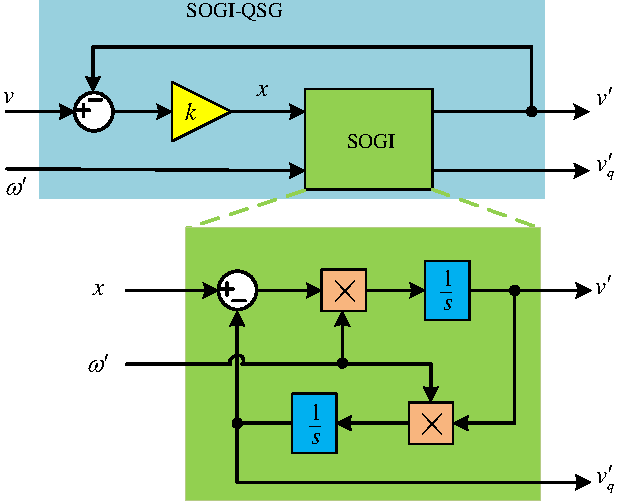
\includegraphics[scale=1]{figures/Chapter_3/Mine/SOGI-OSG.pdf}
	\caption{General structure for SOGI based QSG}
	\label{fig3.1}
\end{figure}
\vspace*{-0.8cm}
A general structure for SOGI based QSG is shown in Fig.\,\ref{fig3.1}. The transfer functions of input signal ($v$) to its in-phase filtered signal ($v^{\prime}$), and input signal ($v$) to its filtered quadrature signal ($v^{\prime}_{q}$) are respectively given in \eqref{3.1} and \eqref{3.2}.
\begin{equation} \label{3.1}
	%\begin{cases}
		\begin{aligned}
			\frac{v^{\prime}(s)}{v(s)} &= \frac{k\omega^{\prime} s}{s^{2} + k\omega^{\prime} s + \omega^{\prime^{2}}} \\
			\Big|\frac{v^{\prime}}{v}\Big| &= \frac{k\omega^{\prime}\omega}{\sqrt{(\omega^{\prime^{2}}-\omega^{2})^{2} + (k\omega^{\prime}\omega)^{2}}} \\
			\angle{\frac{v^{\prime}}{v}}  &= \frac{\pi}{2} - tan^{-1}\Big(\frac{k\omega^{\prime}\omega}{(\omega^{\prime^{2}}-\omega^{2})^{2}}\Big)
		\end{aligned}
	%\end{cases}
\end{equation}
\begin{equation} \label{3.2}
	%\begin{cases}
		\begin{aligned}
			\frac{v^{\prime}_{q}(s)}{v(s)} &= \frac{k\omega^{\prime^{2}}}{s^{2} + k\omega^{\prime} s + \omega^{\prime^{2}}} \\
			\Big|\frac{v^{\prime}_{q}}{v}\Big| &= \frac{ k\omega^{\prime^{2} } }{\sqrt{(\omega^{\prime^{2}}-\omega^{2})^{2} + (k\omega^{\prime}\omega)^{2}}} \\
			\angle{ \frac{ v^{\prime}_{q} } {v} } &= - tan^{-1}\Big(\frac{k\omega^{\prime}\omega}{(\omega^{\prime^{2}}-\omega^{2})^{2}}\Big)
		\end{aligned}
	%\end{cases}	
\end{equation} 
Where, $\omega^{\prime}$ is the resonant or natural frequency of the system, $\omega$ is the frequency of input signal, and $k$ is the gain which decides the transient response of a system. It is evident from \eqref{3.1} and \eqref{3.2} that SOGI-QSG offers band pass and low pass filtering features for $v^{\prime}$ and $v^{\prime}_{q}$, respectively. Furthermore, few more conclusions are derived from \eqref{3.1} and \eqref{3.2} as follows:
%\vspace*{-0.3cm}
\begin{itemize}
	\item Discrepancy between resonant frequency and the fundamental frequency of input signal doesn't meet the requirement of SOGI-QSG in accurately extracting the fundamental frequency signal and its quadrature signal. To address this limitation and achieve frequency adaptability, SRF-PLL is employed in conjunction with the SOGI-QSG, as depicted in Fig.\,\ref{fig3.2}. The SRF-PLL estimates the fundamental frequency of the input signal and provides it as the resonant frequency input to the SOGI-QSG \cite{1712059}. This integration of the SRF-PLL enables the SOGI-QSG to dynamically adjust and align its resonant frequency with the fundamental frequency of the input signal, thereby ensuring accurate extraction of the fundamental frequency signal and its quadrature signal.
	%\vspace*{-0.3cm}
	\item The bandpass filtering characteristic of the SOGI-QSG allows it to selectively pass signals at the resonant frequency while attenuating other frequency signals. Consequently, when applied to a distorted grid with dominant lower-order harmonics, the output signal $v^{\prime}$ of the SOGI-QSG exhibits a non sinusoidal shape. This distortion in the waveform introduces errors in both phase angle and frequency estimation when $v^{\prime}$ is used as an input to the SRF-PLL. Further, the SOGI-QSG is capable of completely removing the DC component of the input signal in the output signal $v^{\prime}$.
	%\vspace*{-0.3cm}
	\item The SOGI-QSG exhibits a low-pass filtering characteristic for the filtered quadrature signal, $v^{\prime}_{q}$. This means that it allows signals with frequencies up to the resonant frequency to pass through, while attenuating signals with frequencies beyond the resonant frequency. Consequently, when applied to a distorted grid voltage containing dominant lower-order harmonics, the resulting $v^{\prime}_{q}$ waveform may exhibit a non sinusoidal shape. In addition to the distortions caused by the lower-order harmonics, the presence of DC signal in the sensed grid voltages, which can arise due to voltage sensor errors, further distorts the $v^{\prime}_{q}$ waveform. This distortion introduces errors in both phase angle and frequency estimation when the distorted $v^{\prime}_{q}$ is utilized as an input to the SRF-PLL.
	%\vspace*{-0.3cm}
	\item $v^{\prime}_{q}$ always lags $v^{\prime}$ by $90^{\circ}$ irrespective of the resonant frequency and gain $k$ \cite{4153695}. 
\end{itemize}
\begin{figure}[]   
	\centering
	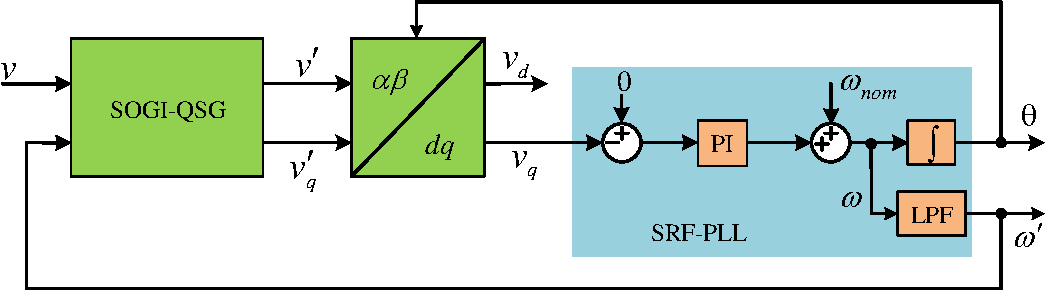
\includegraphics[scale=0.7]{figures/Chapter_3/Mine/SOGI-PLL.pdf}
	\caption{General structure for frequency adaptive 1-ph SOGI-PLL}
	\label{fig3.2}
\end{figure} \vspace*{-0.5cm}
In a three-phase system, three individual SOGI-QSGs are utilized, with one dedicated to each phase. These SOGI-QSGs are responsible for extracting the fundamental frequency signal and its orthogonal signal for each respective phase. The extracted signals are then used to calculate the FFPS components based on the ISCT, as described in \eqref{3.3}. These FFPS components are subsequently fed into the SRF-PLL as shown in Fig.\,\ref{fig3.3}. The calculation of FFPS components are shown in figure inside the positive sequence components (PSC$_{abc}$) blockset.
\begin{equation} \label{3.3}
	%\begin{cases}
		\begin{aligned}
			v^{\prime^{+}}_{a} &= \frac{1}{3} \bigg[ \Big\{ v^{\prime}_{a} - \frac{1}{2} ( v^{\prime}_{b} + v^{\prime}_{c} )   \Big\}  - \frac{\sqrt{3}}{2} \Big\{ v^{\prime}_{bq} -v^{\prime}_{cq}  \Big\} \bigg] \\
			v^{\prime^{+}}_{b} &= - v^{\prime^{+}}_{a} - v^{\prime^{+}}_{c} \\
			v^{\prime^{+}}_{c} &= \frac{1}{3} \bigg[ \Big\{ v^{\prime}_{c} - \frac{1}{2} ( v^{\prime}_{a} + v^{\prime}_{b} )   \Big\}  - \frac{\sqrt{3}}{2} \Big\{ v^{\prime}_{aq} -v^{\prime}_{bq}  \Big\} \bigg] 
		\end{aligned}
	%\end{cases}	
\end{equation}
\begin{figure}[]   
	\centering
	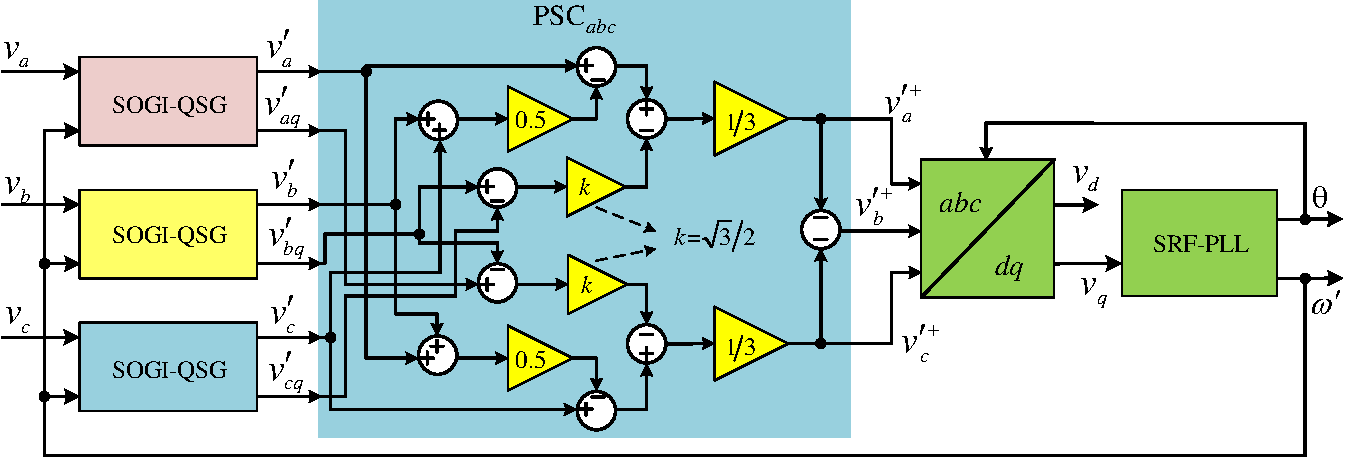
\includegraphics[scale=0.65]{figures/Chapter_3/Mine/SOGI-PLL-3ph.pdf}
	\caption{General structure for frequency adaptive 3-ph SOGI-PLL}
	\label{fig3.3}
\end{figure}
\begin{figure}[]   
	\centering
	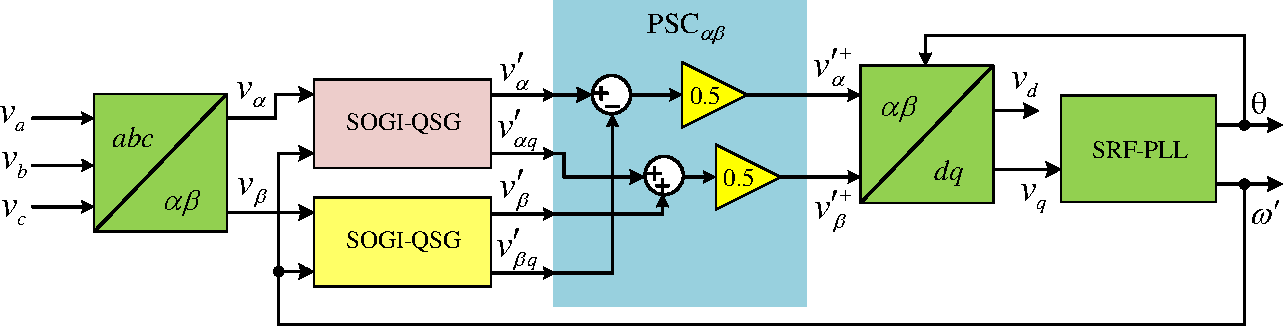
\includegraphics[scale=0.65]{figures/Chapter_3/Mine/DSOGI-PLL.pdf}
	\caption{General structure for frequency adaptive DSOGI-PLL}
	\label{fig3.4}
\end{figure} 
By analyzing system signals in the $\alpha\beta$ reference frame, the number of required SOGI-QSGs can be reduced to two, resulting in a dual SOGI (DSOGI) based PLL. This approach is depicted in Fig.\,\ref{fig3.4}. This configuration also helps to estimate phase angle even in the presence of DC offsets. The zero sequence components or DC offsets in the three-phase input signals are not fed to SOGI operators, thereby DSOGI is insensitive to the DC offsets. The positive sequence components in the $\alpha\beta$ reference frame (PSC$_{\alpha \beta}$) can also be obtained using the ISCT, which is expressed as follows \cite{1712059}.
\begin{equation} \label{3.3a}
	%\begin{cases}
		\begin{aligned}
			v^{\prime^{+}}_{\alpha} &= \frac{1}{2} \Big( v^{\prime}_{\alpha} - v^{\prime}_{\beta q}  \Big) \\
			v^{\prime^{+}}_{\beta} &= \frac{1}{2} \Big( v^{\prime}_{\alpha q} + v^{\prime}_{\beta}  \Big)
		\end{aligned}
	%\end{cases}	
\end{equation} 
In power systems, it is often necessary to extract specific harmonic frequency signals for fault analysis and designing control systems like PR controllers for custom power devices. To meet this requirement, a multiple SOGI (MSOGI) based PLL is employed, as illustrated in Fig.\,\ref{fig3.5} \cite{4758048,5446347}. 

Each SOGI-QSG within the MSOGI is responsible for extracting a particular harmonic frequency signal. However, it is crucial to ensure that the SOGI-QSG intended for a specific harmonic frequency does not receive signals with frequencies lower than that particular harmonic. This is because SOGI-QSG employs a low-pass filter for the quadrature signal ($v^{\prime}_{q}$). Fig.\,\ref{fig3.5} demonstrates this concept, where the input signal for SOGI-QSG-7 is obtained by subtracting the outputs of the preceding SOGI-QSGs (corresponding to $h = 1$ and $5$) from the actual input signal. It should be noted that if the actual input signal contains any of the $2^{nd}, 3^{rd}, 4^{th}$, or $6^{th}$ harmonic frequencies, the extracted $7^{th}$ harmonic frequency signal will not be accurate. This discrepancy arises due to the lowpass filter characteristics of the SOGI.
\begin{figure}[]   
	\centering
	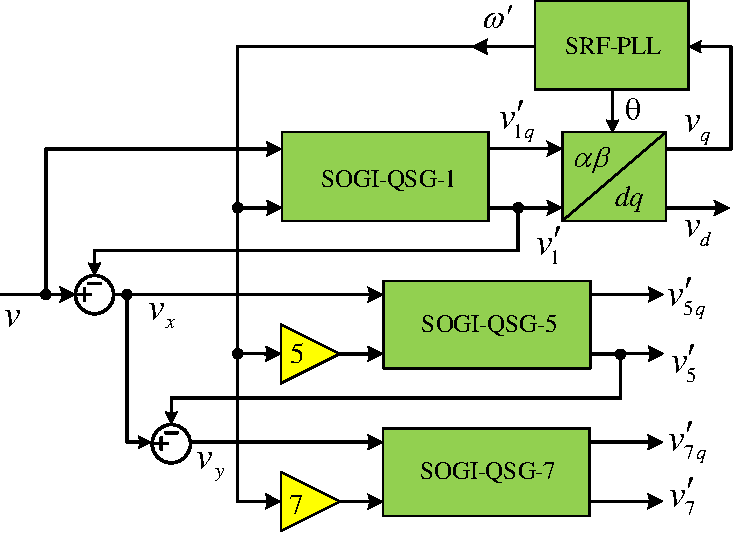
\includegraphics[scale=0.7]{figures/Chapter_3/Mine/MSOGI-PLL.pdf}
	\caption{General structure for frequency adaptive 1-ph MSOGI-PLL}
	\label{fig3.5}
\end{figure} 

Furthermore, the bandpass filter characteristics of the SOGI result in the output of each SOGI-QSG-h predominantly containing the $h^{th}$ harmonic frequency signals, along with partial components of other frequencies. For instance, in Fig.\,\ref{fig3.5}, the output of SOGI-QSG-1 includes the fundamental frequency component, as well as a fraction of the $5^{th}$ and $7^{th}$ harmonic frequency components. As a result, this inaccurate input signal affects the performance of subsequent SOGI-QSG-hs (for $h = 5$ and $7$). To mitigate this issue to some extent, the input signal for each SOGI-QSG is calculated by subtracting the output of all other SOGI-QSGs from the original input signal \cite{4758048,5446347}. This approach helps minimize the undesired components and enhances the accuracy of the extracted harmonic frequency signals.

\vspace*{-1cm}
\subsection{Cascaded Delayed Signal Cancellation Based PLL}
%\vspace*{-0.3cm}
To eliminate a specific frequency signal $v_h(t)$ from a given signal, the delayed signal cancellation (DSC) operator is used \cite{5443553}. The out-of-phase signal of $v_h(t)$ can be obtained by introducing a time delay of $\frac{T}{n}$, where $T$ is the fundamental time period and $n$ is an integer. By adding the given signal to the delayed signal as given below, the specific frequency signal can be eliminated from the given signal.
\begin{equation*} \label{3.4}
DSC_{n} = \frac{1}{2} \big[ v_{h}(t) + v_{h} ( t-T/n ) \big]
\end{equation*}
The choice of the delay time $\frac{T}{n}$ depends on the specific frequency signal to be eliminated. The minimum time delay required for the DSC$_{\text{n}}$ operator is the period from time $t = 0$ to the time at which the negative zero crossing of the signal occurs. In general, the possible delay times $\big(\frac{T}{n}\big)$ to eliminate the $h^{th}$ harmonic frequency signal can be calculated as follows:
\begin{equation} \label{3.5}
\frac{T}{n} = \frac{T}{2h} + k\frac{T}{h} \hspace{1cm} \forall ~~ k < h-0.5 ~~\& ~~ k ~ \epsilon ~ N_{0}.
\end{equation}
For example, to eliminate a $4^{th}$ harmonic frequency signal, the possible delay times are $\frac{T}{8}, \left(\frac{T}{8} + \frac{T}{4}\right), \left(\frac{T}{8} + \frac{2T}{4}\right),$ and $\left(\frac{T}{8} + \frac{3T}{4}\right)$, as shown in Fig.\,\ref{fig3.6}.
\begin{figure}[h]  
	\centering
	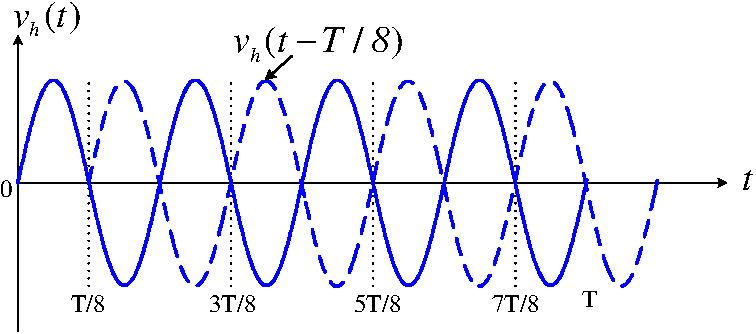
\includegraphics[scale=0.7]{figures/Chapter_3/Mine/DSC.pdf}
	\caption{Fourth order frequency signal and its delayed signal}
	\label{fig3.6}
\end{figure} 

\vspace*{-0.7cm}
In other words, for a known delay time, all the eliminated harmonic signals are obtained from \eqref{3.5} and is given as, \vspace*{-0.5cm}
\begin{equation*} \label{3.6}
h = nk + \frac{n}{2} \hspace{1cm} \forall ~~ k,h ~ \epsilon ~ N_{0}.
\end{equation*}
Based on the above equation, the harmonics eliminated by the DSC operators $DSC_{2}, DSC_{4}, DSC_{8}, DSC_{16} $ and $ DSC_{32} $ are $ 2k+1$, $4k+2, 8k+4, 16k+8 $ and $32k+16$, respectively. These operators are commonly used because they ensure that no single harmonic signal is eliminated by any two operators. The harmonics that are passed without attenuation through these DSC operators are $2k, 4k, 8k, 16k$ and $32k$, respectively. To eliminate all lower order harmonics effectively, these DSC operators are cascaded in such a way that no signal is attenuated by any individual DSC operator. This results in a new operator called the cascaded delayed signal cancellation $(CDSC)$ operator \cite{5624643,5668509,6249751,5959976,7081338,8624618}. It is important to note that while this operator is designed for use in the $dq$ reference frame, if applied in the $abc$ frame, it will eliminate the fundamental frequency component that is necessary for grid synchronization using an SRF-PLL. 
%\vspace*{-0.5cm}
\begin{table*}[ht] 
	\centering
	\captionof{table}{Harmonic order and nature in $abc$ and $dq$ frames at a rotating speed of $\omega$}
	\label{table3.1}
	\begin{tabular}{|c|c|c|c|c|} 
		\hline
		\multicolumn{3}{|c|}{\footnotesize \textbf{Harmonic order \boldmath$(h)$ in \boldmath$abc$ frame ~ $\forall ~~ k ~ \epsilon ~ N_{0}$ }} &  \multicolumn{2}{|c|}{\footnotesize \textbf{Harmonic order \boldmath$(h)$ in \boldmath$dq$ frame ~ $\forall ~~ k ~ \epsilon ~ N_{0}$ }} \\
		\hline
		\footnotesize \boldmath$h$ & \footnotesize \textbf{sequence} & \footnotesize \textbf{nature} & \footnotesize \boldmath$h$ & \footnotesize \textbf{nature} \\
		\hline
		\multirow{2}{*}{\footnotesize $6k + 1$} & \multirow{2}{*}{\footnotesize positive} & \footnotesize odd, balanced & \footnotesize $6k$ & \multirow{2}{*}{\footnotesize even} \\ 
		\cline{3-4}
		&  & \footnotesize odd, unbalanced & \footnotesize $6k ~ \& ~ 6k+2$ &  \\
		\hline
		\multirow{2}{*}{\footnotesize $6k - 1$} & \multirow{2}{*}{\footnotesize negative} & \footnotesize odd, balanced & \footnotesize $6k$ & \multirow{2}{*}{\footnotesize even} \\ 
		\cline{3-4}
		&  & \footnotesize odd, unbalanced & \footnotesize $6k ~ \& ~ 6k-2$ &  \\
		\hline
		\multirow{2}{*}{\footnotesize $3(2k + 1)+1$} & \multirow{2}{*}{\footnotesize positive} & \footnotesize even, balanced & \footnotesize $3(2k+1)$ & \multirow{2}{*}{\footnotesize odd} \\ 
		\cline{3-4}
		&  & \footnotesize even, unbalanced & \footnotesize $3(2k+1) ~ \& ~ 3(2k+1)+2$  &  \\
		\hline
		\multirow{2}{*}{\footnotesize $3(2k - 1)-1$} & \multirow{2}{*}{\footnotesize negative} & \footnotesize even, balanced & \footnotesize $3(2k+1)$ & \multirow{2}{*}{\footnotesize odd} \\ 
		\cline{3-4}
		&  & \footnotesize even, unbalanced & \footnotesize $3(2k+1) ~ \& ~ 3(2k+1)-2$  &  \\
		\hline
		\multirow{2}{*}{\footnotesize $3k ~~\forall ~ k ~ \epsilon ~ N$} & \multirow{2}{*}{\footnotesize zero} & \footnotesize odd/even, balanced & \multicolumn{2}{|c|}{\footnotesize No $dq$ components present} \\ 
		\cline{3-5}
		&  & \footnotesize odd/even, unbalanced & \footnotesize $3k+1 ~ \& ~ 3k-1$ & \footnotesize even/odd  \\
		\hline
		\multirow{2}{*}{\footnotesize $0$} & \multirow{2}{*}{$-$} & \footnotesize DC, balanced & \multicolumn{2}{|c|}{\footnotesize No $dq$ components present} \\ 
		\cline{3-5}
		&  & \footnotesize DC, unbalanced & \footnotesize $+1 $ & \footnotesize odd  \\
		\hline
	\end{tabular} 
\end{table*}\vspace*{-0.5cm}

The $dq$ reference frames in vector space have the flexibility to be rotated at any frequency and in any direction. Typically, they are rotated at the fundamental frequency and in synchronism with the rotation of the resultant vector. As a result, the balanced fundamental frequency components in the $abc$ frame appear as a DC quantity in the $dq$ frame.

Table \ref{table3.1} provides the relationship between the harmonic orders in the $abc$ and $dq$ frames. It can be observed that odd-order frequency signals in the $abc$ frame appear as even-order harmonics in the $dq$ frame, and vice versa. The $CDSC_{2,4,8,16,32}$ operator in the $dq$ frame passes all $32k$ harmonic order frequency signals, corresponding to harmonic order signals of $32k\pm1$ in the $abc$ frame. Therefore, the $CDSC_{2,4,8,16,32}$ operator in the $dq$ frame effectively extracts the equivalent fundamental frequency component in the $abc$ frame .

The total delay time of the $CDSC_{2,4,8,16,32}$ operator is $31T/32$. To reduce the total delay time to $15T/16$, a $CDSC_{2,4,8,16}$ operator is used. However, the $CDSC_{2,4,8,16}$ operator fails to eliminate all $16k$ harmonic frequency signals in the $dq$ frame, corresponding to harmonic order signals of $16k\pm1$ in the $abc$ frame. As a result, when the $CDSC_{2,4,8,16}$ operator is fed to the SRF-PLL for grid synchronization, a lower bandwidth SRF-PLL is required compared to when $CDSC_{2,4,8,16,32}$ operator is fed to the SRF-PLL.

Additionally, the CDSC operator in the $dq$ frame introduces a time delay into the control loop of the SRF-PLL. This in-loop delay can have an adverse effect on the dynamic performance of the PLL. To ensure high stability of the SRF-PLL, the equivalent of the CDSC operator in the $dq$ frame should be relocated into the $\alpha\beta$ frame using the following expression \cite{5668509}.
\begin{equation} \label{3.25}
	\begin{bmatrix}
		DSC_{n}[ v_{\alpha h} ]\\
		DSC_{n}[ v_{\beta h} ]
	\end{bmatrix}
	= 
	\begin{bmatrix}
		cos\,h^{*}\theta & -sin \,h^{*}\theta\\
		sin \,h^{*}\theta & cos \,h^{*}\theta
	\end{bmatrix}
	*
	\begin{bmatrix}
		DSC_{n}[ v_{dh} ]\\
		DSC_{n}[ v_{qh} ]
	\end{bmatrix}
\end{equation} 
where, $DSC_{n}[ v_{dqh} ] = \frac{1}{2} \big[ v_{dq}h(\omega t) + v_{dq} h( \omega t-T/n ) \big]$, $\omega$ is the fundamental angular frequency, $h$ is the harmonic order, $h^{*} = \pm \, h$ is the required positive sequence harmonic frequency component to be extracted by the CDSC operator. The positive sign `$+$' is used for positive sequence signals, while the negative sign `$-$' is used for negative sequence signals. The variable $\theta$ is defined as $\theta = \omega t$. The simplified expression of \eqref{3.25} can be written as below.
\vspace*{-0.5cm}
\begin{equation} \label{3.26} 
\begin{bmatrix}
DSC_{n}[ v_{\alpha h} ]\\ %\vspace*{0.2cm}
DSC_{n}[ v_{\beta h} ]
\end{bmatrix}
= \frac{1}{2}
\begin{bmatrix}
v_{\alpha} h(\omega t) + v_{\alpha} h(\omega t - \frac{T}{n}) \cos \frac{2\pi h^{*}} { n }  - v_{\beta} h(\omega t - \frac{T}{n}) \sin \frac{2\pi h^{*}} { n }  \\%\vspace*{0.2cm}  
v_{\beta} h(\omega t) + v_{\beta} h(\omega t - \frac{T}{n}) \cos \frac{2\pi h^{*}} { n } + v_{\alpha} h(\omega t - \frac{T}{n}) \sin \frac{2\pi h^{*}} { n }
\end{bmatrix}
\end{equation}
\begin{figure}[h]  
	\centering
	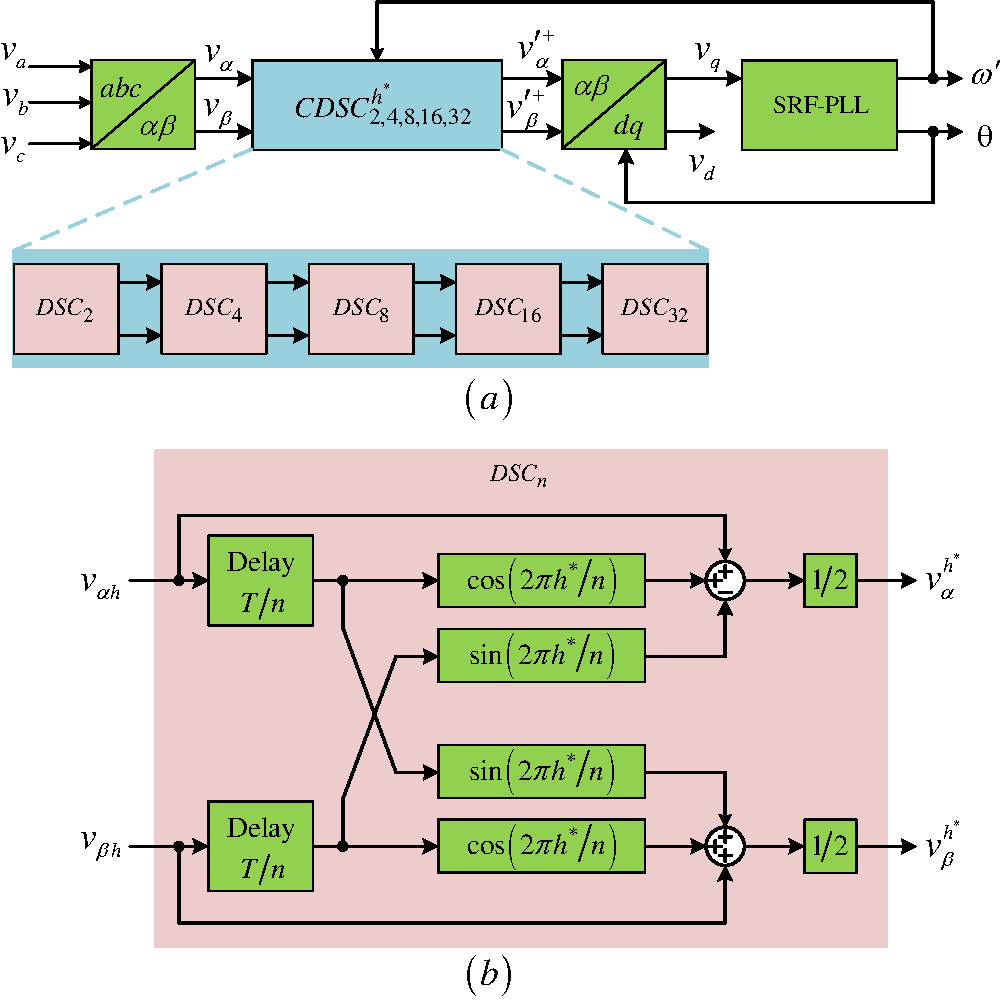
\includegraphics[scale=0.7]{figures/Chapter_3/Mine/DSC-CDSC-PLL.pdf}
	\caption{(a) General structure for frequency adaptive 3-ph CDSC-PLL, and (b) Time domain implementation of $DSC_{n}$ operator}
	\label{fig3.7}
\end{figure}

The CDSC operator is known for its efficiency in execution, as it involves simple operations such as transport delay, multiplication, and summation in the digital controller. However, it may encounter a small discretization error when non-integer samples are used for the delay operation in any DSC operator \cite{5624643,5959976}. To obtain integer samples for the delay operation, the total number of samples in a fundamental time period $T$ must be chosen as an integer multiple of 32. In many applications, including aircraft power systems, the fundamental time period $T$ is not constant and needs to be continuously updated for accurate delay operation. This update is achieved using a SRF-PLL, as depicted in Fig.\,\ref{fig3.7}. However, the updating of $T$ may result in non-integer samples in the delay operation, leading to small discretization errors. To mitigate this discretization error and enhance the performance of CDSC, a linear interpolation method is proposed in \cite{5624643}.

To transform the CDSC operator into a quadrature signal generator (QSG) suitable for single-phase systems, the concept of anticonjugate decomposition (ACD) is introduced in \cite{6276263}. By utilizing this approach, the $\alpha$ component of the CDSC input is set to $0$, while the actual single-phase signal is assigned to the $\beta$ component. Consequently, the desired frequency signal and its quadrature signals are obtained at the $\beta$ and $\alpha$ output terminals of the CDSC, respectively, with a 50\% attenuation. This ACD-based CDSC configuration enables its application in single-phase systems, and the corresponding general diagram is illustrated in Fig.\,\ref{fig3.8}.
\begin{figure}[h]  
	\centering
	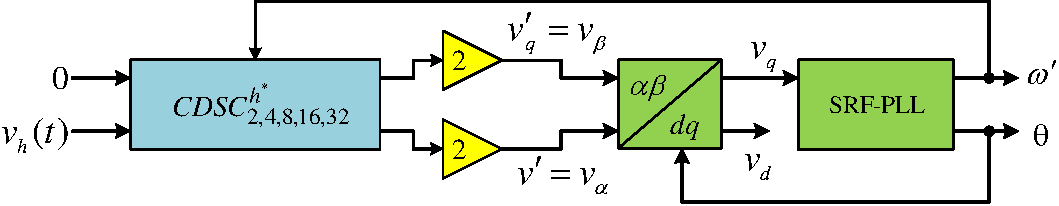
\includegraphics[scale=0.7]{figures/Chapter_3/Mine/ACD-CDSC-PLL.pdf}
	\caption{General structure for frequency adaptive 1-ph ACD-CDSC-PLL}
	\label{fig3.8}
\end{figure} 

%For three phase system applications, the ACD based CDSC shown in  Fig.9., 
%is used on each phase and obtained fundamental component as well as its quadrature signals of each phase. From these signals, positive sequence components are extracted using ISC theory and fed to SRF-PLL as in the case of SOGI based PLL. To reduce the number of CDSC operators, the ACD based dual CDSC (ACD-DCDSC) shown in Fig.10., is proposed. 
%\vspace*{-0.3cm}
\subsection{Multiple Delayed Signal Cancellation Based PLL} 
The MDSC operator, introduced in \cite{8274027}, offers a reduced delay time and storage requirement compared to the CDSC operator. The MDSC operator delays the test signal multiple times using various delay times in such a way that the sum of the test signal and the delayed signals becomes zero. These delay times are chosen as integer multiples of $T/15$, ensuring that the delay does not exceed the fundamental time period $T$. The resulting operator, denoted as $MDSC_{15}$, has a total delay time of $14T/15$, which is shorter than the delay time of $CDSC_{2,4,8,16}$.

In the $dq$ frame, the $MDSC_{15}$ operator eliminates all harmonic frequency signals except the $15k$ frequency signals, which correspond to $15k\pm1$ frequency signals in the $abc$ frame. Notably, $MDSC_{15}$ passes lower-order harmonics of 14 and 16, which are even, whereas $CDSC_{2,4,8,16}$ passes odd harmonics of 15 and 17. Given that even harmonics are typically absent in power system applications, the bandwidth of the SRF-PLL can be chosen to be higher for $MDSC_{15}$ compared to $CDSC_{2,4,8,16}$, providing greater flexibility in SRF-PLL design.

The $dq$ equivalent of $MDSC_{15}$ operator can be transformed onto the $\alpha\beta$ frame using the below equation. 
%\begin{figure}[h] 
%	\centering
%	\includegraphics[scale=0.4]{Freq-Variation-results.pdf}
%	\caption{General structure for frequency adaptive 1-ph ACD-CDSC-PLL.}
%	\label{fig10}
%\end{figure}
\begin{equation} \label{3.27} 
	\begin{bmatrix}
		MDSC_{15}[ v_{\alpha h} ]\\
		MDSC_{15}[ v_{\beta h} ]
	\end{bmatrix}
	= 
	\begin{bmatrix}
		cos \,h^{*}\theta & -sin \,h^{*}\theta\\
		sin \,h^{*}\theta & cos \,h^{*}\theta
	\end{bmatrix}
	\begin{bmatrix}
		MDSC_{15}[ v_{dh} ]\\
		MDSC_{15}[ v_{qh} ]
	\end{bmatrix}
\end{equation} 
Where, $$MDSC_{15}[ v_{dqh} ] = \frac{1}{15} \sum_{l=0}^{14} \big[ v_{dq} h( \omega t-Tl/15 ) \big].$$
The above expression is simplified as given below. 
\begin{equation} \label{3.28} 
\begin{bmatrix}
MDSC_{15}[ v_{\alpha h} ] \\%\vspace*{0.2cm}\\
MDSC_{15}[ v_{\beta h} ]
\end{bmatrix}
= \frac{1}{15}
\begin{bmatrix}
v_{\alpha} h(\omega t) + \sum\limits_{l=0}^{14} \Big\{v_{\alpha} h(\omega t - \frac{Tl}{15}) \cos \frac{2\pi h^{*}l} { 15 }  - v_{\beta} h(\omega t - \frac{Tl}{15}) \sin \frac{2\pi h^{*}l} { 15 } \Big\}  \\ %\vspace*{0.2cm} \\ 
v_{\beta} h(\omega t) + \sum\limits_{l=0}^{14} \Big\{ v_{\beta} h(\omega t - \frac{Tl}{15}) \cos \frac{2\pi h^{*}l} { 15 } + v_{\alpha} h(\omega t - \frac{Tl}{15}) \sin \frac{2\pi h^{*}l} { 15 } \Big\}
\end{bmatrix}
\end{equation}

\section{PERFORMANCE EVALUATION OF ADVANCED PLLs}
\begin{figure}[] 
	\centering
	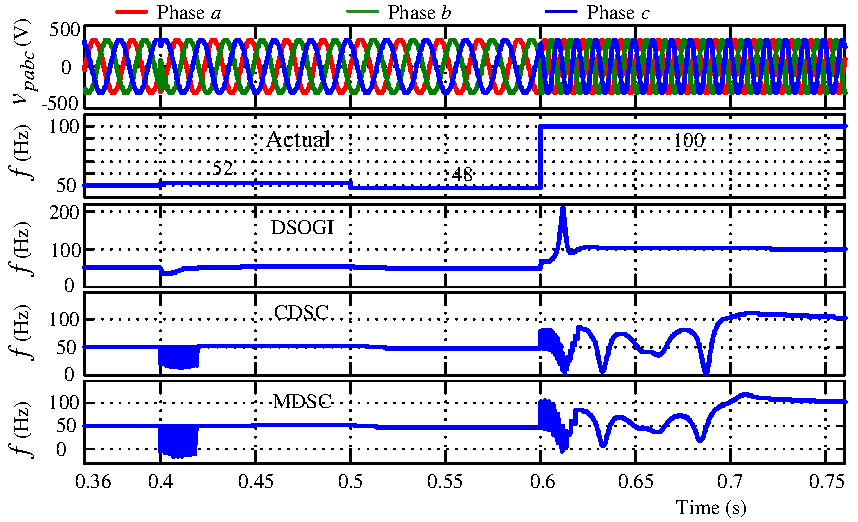
\includegraphics[scale=1]{figures/Chapter_3/Mine/SimRes1_new.pdf}
	\caption{Simulation results: Frequencies of advanced PLLs under grid frequency variations}
	\label{fig3.9(1)}
\end{figure}
To assess the individual performance of the DSOGI, CDSC$_{2,4,8,16}$, and MDSC$_{15}$ operators under different grid conditions, MATLAB simulations are conducted with the same bandwidth settings for their respective SRF-PLLs. The evaluation of these advanced PLLs is primarily based on the accuracy of tracking the frequency, $f$ in the SRF-PLL. A high-quality PLL is characterized by zero steady-state error in the phase angle extracted by the PLL when subjected to a ripple-free frequency input applied to the PLL's integrator. The performance evaluation aims to determine the ability of these advanced PLLs to achieve precise frequency tracking with minimal error.
\subsection{Frequency Jump} 
%\vspace*{-0.3cm}
The frequency of the system is manipulated in the simulation to evaluate the performance of the DSOGI, CDSC$_{2,4,8,16}$, and MDSC$_{15}$ PLLs. Initially, the frequency is increased from $50\,\si{Hz}$ to $52\,\si{Hz}$ at $t=0.4\,\si{s}$, then it is decreased to $48\,\si{Hz}$ at $t=0.5\,\si{s}$, and finally, it rapidly rises to $100\,\si{Hz}$ at $t=0.6\,\si{s}$, as depicted in Fig.\,\ref{fig3.9(1)}.

Analyzing the frequency variation of the PLLs, it can be observed that for a significant jump in frequency, all PLLs exhibit good steady-state tracking performance. However, the DSOGI-PLL demonstrates superior tracking speed compared to the other two PLLs. On the other hand, for small changes in frequency, all PLLs exhibit similar tracking accuracy and speed. 
%\vspace*{-0.8cm} 
%\begin{figure}[] 
%	\centering
%	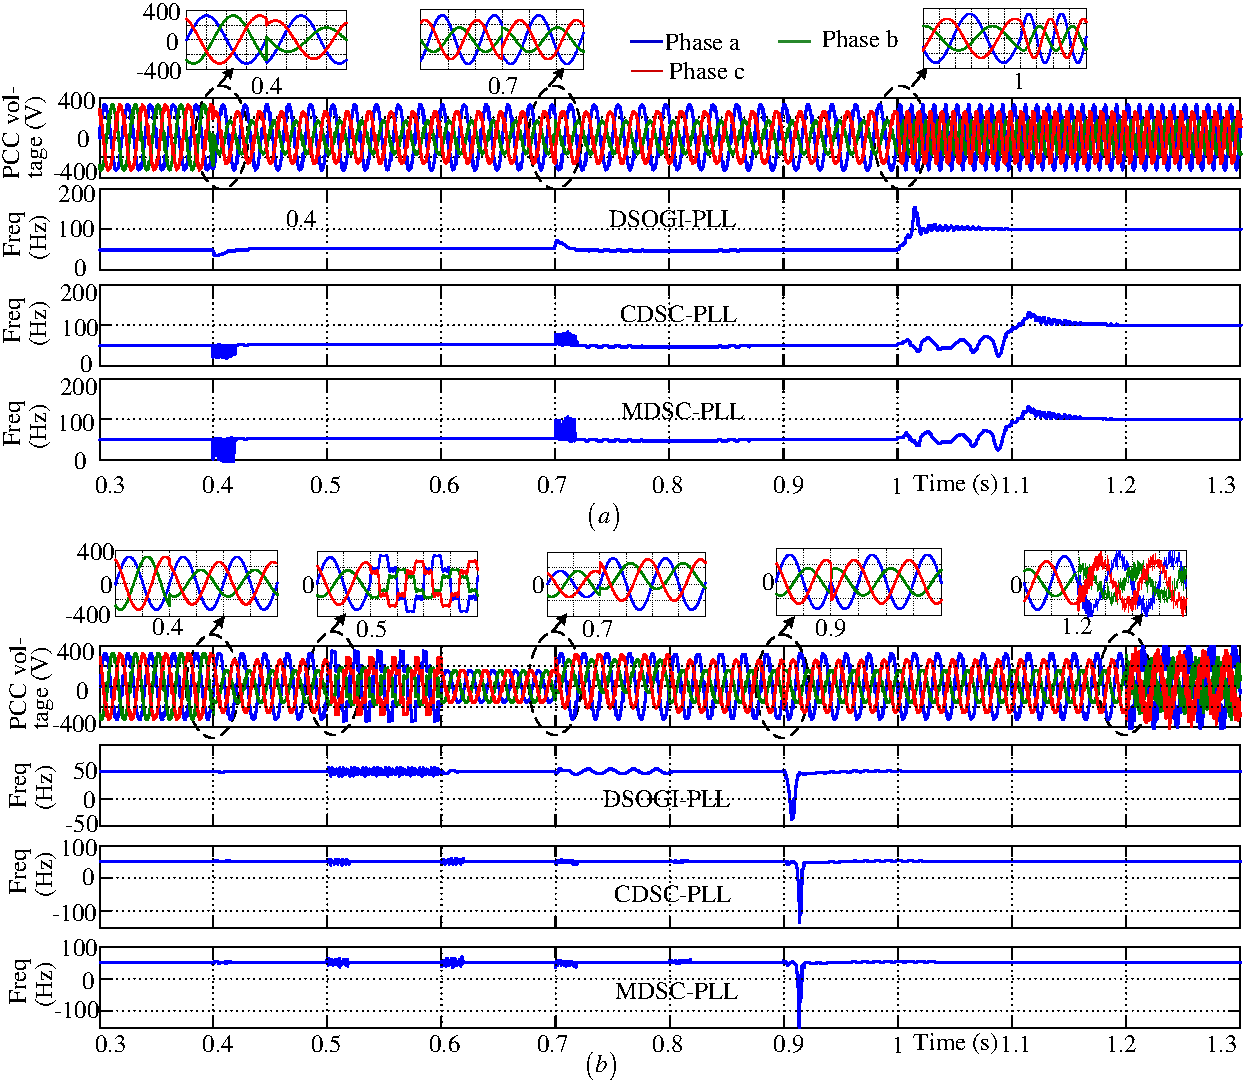
\includegraphics[scale=0.7]{figures/Chapter_3/Mine/various_grid_results.pdf}
%	\caption{Simulation results: Frequencies of advanced PLLs under (a) Grid frequency variations, and (b) Various other grid conditions}
%	\label{fig3.9}
%\end{figure}
\subsection{Voltage Disturbances without Harmonics}
%\vspace*{-0.3cm}
The balanced voltage sag of $0.5\,\si{pu}$ is introduced from time $t=0.4\,\si{s}$ to $t=0.5\,\si{s}$ as shown in Fig.\,\ref{fig3.9(2)}. And, the unbalanced voltage sag is introduced from time $t=0.5\,\si{s}$ to $t=0.6\,\si{s}$ and the per unit voltages of phases $a,b$ and $c$ are respectively $1, 1$ and $0.5$. From the figure, it can be concluded that although all PLLs exhibit good steady-state performance, CDSC and MDSC based PLLs have better transient performance in terms of overshoot and settling time. The similar response is noticed during both balanced and unbalanced voltage swell conditions as shown in Fig.\,\ref{fig3.9(3)}. The balanced voltage swell of $1.2\,\si{pu}$ is introduced at time $t=0.6\,\si{s}$ and the unbalanced voltage swell in phase-$a$ ($v_{pa}=1.2\,\si{pu}$) is introduced at $t=0.7\,\si{s}$.
%\vspace*{-0.5cm}
\begin{figure}[h] 
	\centering
	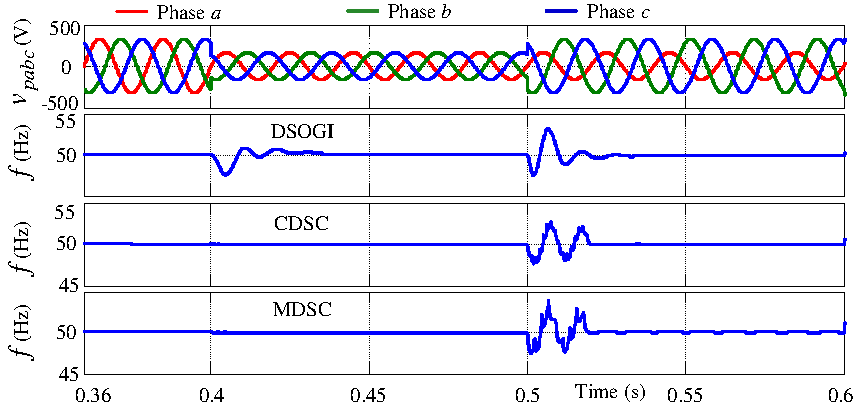
\includegraphics[scale=1]{figures/Chapter_3/Mine/SimRes2_new.pdf}
	\caption{Simulation results: Frequencies of advanced PLLs under voltage sag conditions}
	\label{fig3.9(2)}
\end{figure}
\begin{figure}[h] 
	\centering
	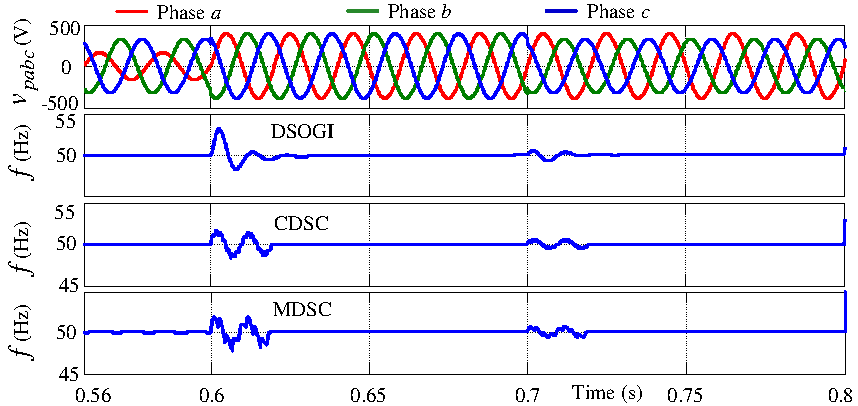
\includegraphics[scale=1]{figures/Chapter_3/Mine/SimRes3_new.pdf}
	\caption{Simulation results: Frequencies of advanced PLLs under voltage swell conditions}
	\label{fig3.9(3)}
\end{figure}
\begin{figure}[h] 
	\centering
	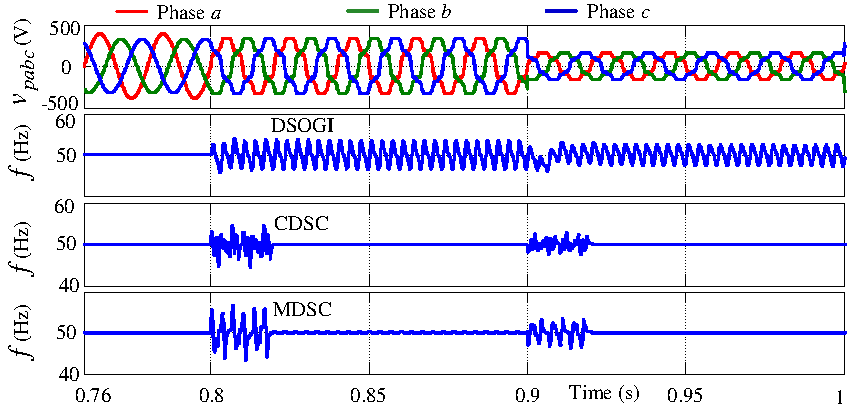
\includegraphics[scale=1]{figures/Chapter_3/Mine/SimRes4_new.pdf}
	\caption{Simulation results: Frequencies of advanced PLLs under balanced voltage sag conditions with harmonics}
	\label{fig3.9(4)}
\end{figure}
\subsection{Voltage Disturbances with Harmonics}
%\vspace*{-0.3cm}
The percentage of unbalance in the fundamental voltage remains the same as in the previous case. Additionally, $5^{th}, 7^{th}, 11^{th}$, and $13^{th}$ harmonics are added to the voltage waveform, resulting in a total harmonic distortion (THD) of approximately $14\%$. This is depicted in Figs.\,\ref{fig3.9(4)}-\ref{fig3.9(6)}. The nominal voltage with harmonics at $t=0.8\,\si{s}$ and balanced voltage sag with harmonics at $t=0.9\,\si{s}$ are introduced, as shown in Fig.\,\ref{fig3.9(4)}. The unbalanced voltage sag with harmonics at $t=1\,\si{s}$ and balanced voltage swell with harmonics at $t=1.1\,\si{s}$ are introduced, as shown in Fig.\,\ref{fig3.9(5)}. The unbalanced voltage swell with harmonics is introduced at $t=1.2\,\si{s}$, as shown in Fig.\,\ref{fig3.9(6)}. In all these cases, the ripple in frequency is observed only for DSOGI, indicating an error in its phase angle tracking. Therefore, the performance of CDSC and MDSC is superior to DSOGI in the presence of harmonics. The CDSC experiences less ripple in magnitude compared to MDSC.
\begin{figure}[] 
	\centering
	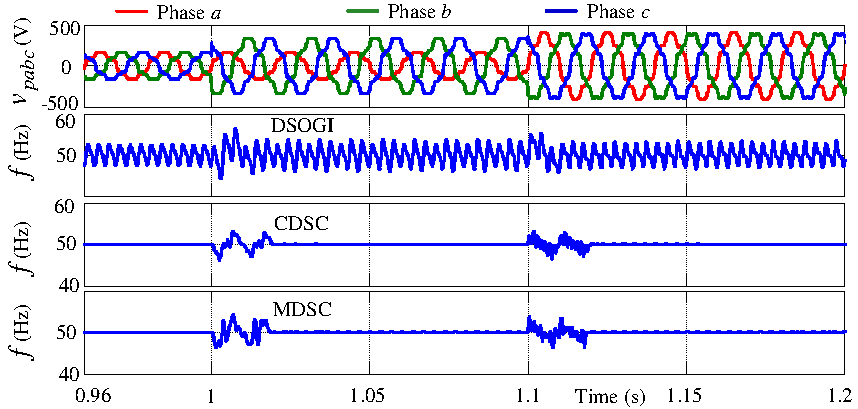
\includegraphics[scale=1]{figures/Chapter_3/Mine/SimRes5_new.pdf}
	\caption{Simulation results: Frequencies of advanced PLLs under unbalanced voltage sag and balanced voltage swell conditions with harmonics}
	\label{fig3.9(5)}
\end{figure}
\begin{figure}[] 
	\centering
	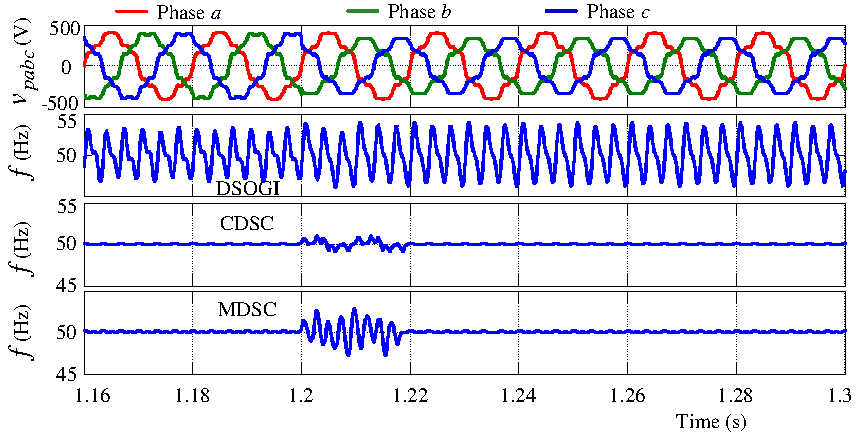
\includegraphics[scale=1]{figures/Chapter_3/Mine/SimRes6_new.pdf}
	\caption{Simulation results: Frequencies of advanced PLLs under unbalanced voltage swell condition with harmonics}
	\label{fig3.9(6)}
\end{figure}
%\vspace*{-0.5cm}
\subsection{Phase Angle Jump}
%\vspace*{-0.3cm}
In the given scenario, a maximum jump in phase angle of $180^\circ$ is set at time $t=0.4\,\si{s}$ as shown in Fig.\,\ref{fig3.9(7)}(a). The enlarged view of Fig.\,\ref{fig3.9(7)}(a) is shown in Fig.\,\ref{fig3.9(7)}(b) to observe the settling time and peak over/undershoot magnitudes. It is observed that all the PLLs exhibit similar response during phase jump. All the PLLs show no ripple in frequency at steady-state. Therefore, the phase angle tracking performance of these PLLs is not affected by the phase angle jump, indicating their ability to accurately track the phase angle under such conditions.
\begin{figure}[] 
	\centering
	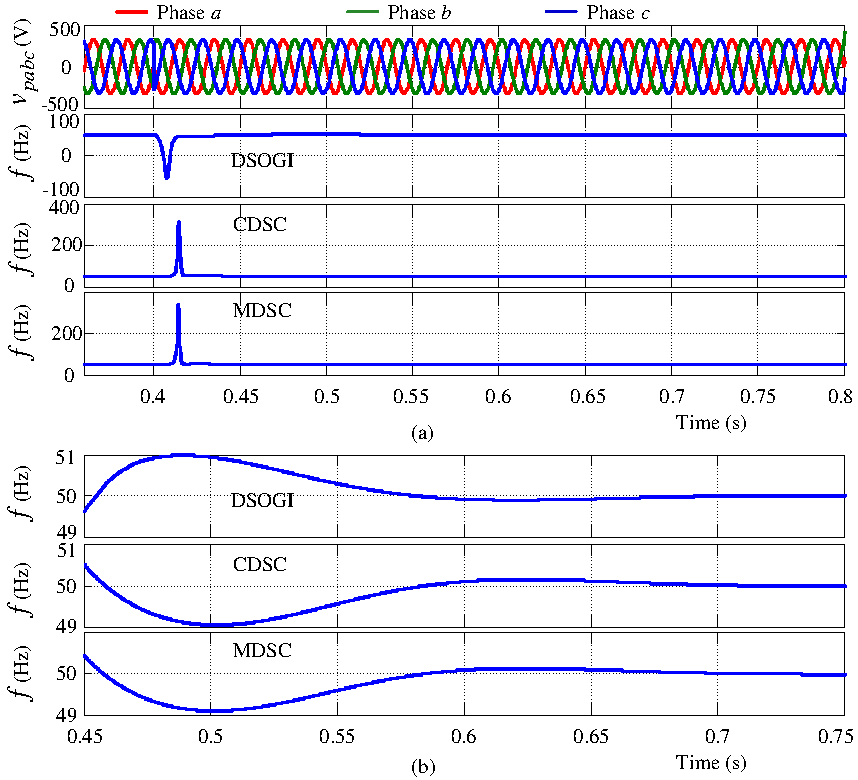
\includegraphics[scale=1]{figures/Chapter_3/Mine/SimRes7_new.pdf}
	\caption{Simulation results: (a) Frequencies of advanced PLLs under voltage phase jump of $180^\circ$, and (b) Enlarged view of (a) }
	\label{fig3.9(7)}
\end{figure}
\begin{figure}[] 
	\centering
	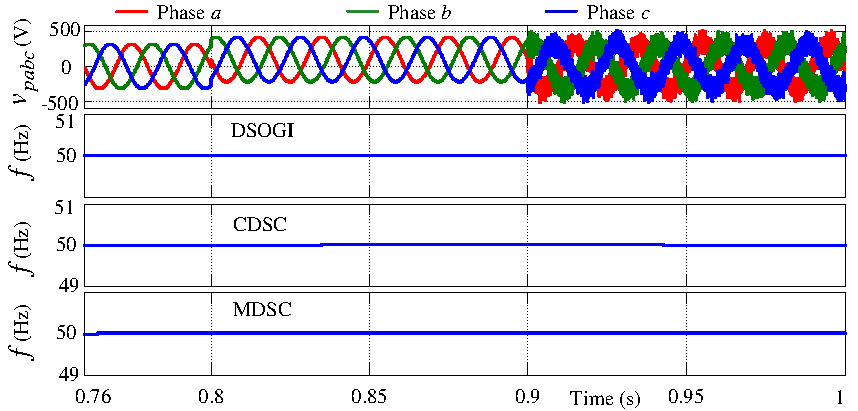
\includegraphics[scale=1]{figures/Chapter_3/Mine/SimRes8_new.pdf}
	\caption{Simulation results: Frequencies of advanced PLLs under voltage with DC offset and voltage distortion conditions}
	\label{fig3.9(8)}
\end{figure}  
\subsection{Presence of DC Components}
%\vspace*{-0.3cm}
In the scenario where the grid voltages are sensed and processed in a controller for power electronic converter control, it is possible for DC components to be added to the sensed values. In this case, the performance of PLLs is evaluated for the presence of DC components in the fundamental balanced voltages, as shown in Fig.\,\ref{fig3.9(8)} from time $t=0.8\,\si{s}$ to $t=0.9\,\si{s}$. It can be observed that all the PLLs provide ripple free frequency, consequently, the performance of all PLLs in tracking the phase angle remains satisfactory even in the presence of DC offsets in the three-phase PCC voltages.
%\vspace*{-0.5cm}
\subsection{Voltage Distortions}
In the given scenario, distorted balanced voltages are applied from time $t=0.9\,\si{s}$ to $t=1\,\si{s}$, as shown in Fig.\,\ref{fig3.9(8)}. It can be observed that the distortions in the voltage waveforms do not have any significant effect on the frequency, as there is no visible ripple in the frequency response of all PLLs. Consequently, the performance of all PLLs in tracking the phase angle remains satisfactory even in the presence of distorted unbalanced voltages.

It is important to note that the change in frequency even during the transients must be within the allowable range. This allowable frequency threshold is generally quite less unlike in this simulation study. However, this study is presented to understand the behavior of three different operators DSOGI, CDSC and MDSC. To limit the frequency change to the allowable threshold, a special attention is required in the design of SRF-PLL but not in the design of these three operators. 
    
\section{SUMMARY}
In this chapter, a comprehensive review of advanced PLLs, including SOGI, CDSC, and MDSC based PLLs, is presented for the accurate extraction of FFPS components. MATLAB simulations are conducted to evaluate the performance of these PLLs under various grid conditions.

The SOGI-based PLL exhibits attenuation of harmonics but fails to completely nullify them, resulting in unsatisfactory phase angle tracking performance in the presence of harmonics and DC components in grid voltages. On the other hand, the CDSC and MDSC based PLLs employ delay operators that are carefully chosen to completely eliminate specific sets of harmonics. As a result, the performance of CDSC and MDSC based PLLs is found to be satisfactory for all grid conditions, as long as the grid does not have dominant harmonics that cannot be eliminated by these PLLs.

Based on these findings, it is concluded that CDSC and MDSC based PLLs are more preferable than SOGI based PLL for power system applications. These advanced PLLs provide improved performance in terms of accurate phase angle tracking, making them suitable choices for custom power devices. In comparison to MDSC, the CDSC operator requires fewer delay operations, making it computationally less intensive. Therefore, the CDSC operator will be employed in the following chapters for controlling custom power devices. 